
\documentclass{article}
\usepackage[headheight=20pt, margin=1.0in, top=1.2in]{geometry}
\usepackage{amsmath, amssymb, amsthm, thmtools, tcolorbox, array, graphicx, makeidx, cancel, multirow, fancyhdr, xypic, color, nicefrac, rotating, multicol, caption, subcaption, xcolor, tikz, tikz-3dplot, tikz-cd, pgfplots, import, enumitem, calc, booktabs, wrapfig, siunitx, hyperref,float}
\hypersetup{colorlinks=true,linkcolor=blue}
\usepackage[all]{xy}
\usepackage{esint}
\setlength{\parindent}{0in}
\sisetup{per-mode = symbol}
\usetikzlibrary{calc,arrows,svg.path,decorations.markings,patterns,matrix,3d,fit}
\usepgfplotslibrary{groupplots}
\pgfplotsset{compat=newest}
\newtcolorbox{mydefbox}[2][]{colback=red!5!white,colframe=red!75!black,fonttitle=\bfseries,title=#2,#1}
\newtcolorbox{mythmbox}[2][]{colback=gray!5!white,colframe=gray!75!black,fonttitle=\bfseries,title=#2,#1}
\newtcolorbox{myexamplebox}[2][]{colback=green!5!white,colframe=green!75!black,fonttitle=\bfseries,title=#2,#1}
\newtcolorbox{mypropbox}[2][]{colback=blue!5!white,colframe=blue!75!black,fonttitle=\bfseries,title=#2,#1}
\declaretheoremstyle[headfont=\color{blue}\normalfont\bfseries,]{colored}
\theoremstyle{definition}
\newtheorem{theorem}{Theorem}
\newtheorem{corollary}[theorem]{Corollary}
\newtheorem{lemma}[theorem]{Lemma}
\newtheorem{proposition}[theorem]{Proposition}
\newtheorem{problem}[theorem]{Problem}
\newtheorem{definition}[theorem]{Definition}
\newtheorem{exercise}[theorem]{Exercise}
\newtheorem{example}[theorem]{Example}
\newtheorem{solution}[theorem]{Solution}
\newtheorem*{thm}{Theorem}
\newtheorem*{lem}{Lemma}
\newtheorem*{prob}{Problem}
\newtheorem*{exer}{Exercise}
\newtheorem*{prop}{Proposition}
\def\R{\mathbb{R}}
\def\F{\mathbb{F}}
\def\Q{\mathbb{Q}}
\def\C{\mathbb{C}}
\def\N{\mathbb{N}}
\def\Z{\mathbb{Z}}
\def\Ra{\Rightarrow}
\def\e{\epsilon}
\newcommand{\typo}[1]{{\color{red}{#1}}}
\newcommand\thedate{\today}
\newcommand{\mb}{\textbf}
\newcommand{\norm}[2]{\|{#1}\|_{#2}}
\newcommand{\normm}[1]{\|#1\|}
\newcommand{\mat}[1]{\begin{bmatrix} #1 \end{bmatrix}}
\newcommand{\eqtext}[1]{\hspace{3mm} \text{#1} \hspace{3mm}}
\newcommand{\set}[1]{\{#1\}}
\newcommand{\inte}{\textrm{int}}
\newcommand{\ra}{\rightarrow}
\newcommand{\minv}{^{-1}}
\newcommand{\tx}[1]{\text{ {#1} }}
\newcommand{\abs}[1]{|#1|}
\newcommand{\mc}[1]{\mathcal{#1}}
\newcommand{\uniflim}{\mathop{\mathrm{unif\lim}}}
\newcommand{\notimplies}{\mathrel{{\ooalign{\hidewidth$\not\phantom{=}$\hidewidth\cr$\implies$}}}}
\pagestyle{fancy}
\fancyhf{}
\fancyhead[L]{Title of the Document}
\fancyhead[C]{}
\fancyhead[R]{\thepage}
\fancyfoot[L]{}
\fancyfoot[C]{}
\fancyfoot[R]{}
\renewcommand{\headrulewidth}{0.4pt}
\renewcommand{\footrulewidth}{0.4pt}
\numberwithin{equation}{section}
% Increase spacing between paragraphs
\setlength{\parskip}{1em}
% Increase spacing before and after sections
\usepackage{titlesec}
\titlespacing*{\section}{0pt}{3ex plus 1ex minus .2ex}{2ex plus .2ex}
\titlespacing*{\subsection}{0pt}{2ex plus 1ex minus .2ex}{1ex plus .2ex}
\titlespacing*{\subsubsection}{0pt}{1ex plus 1ex minus .2ex}{1ex plus .2ex}
\title{\textbf{Title of the Document}}
\author{Author Name}
\date{\today}
\begin{document}
\maketitle
\tableofcontents
\newpage
\section{Exercises}

\begin{enumerate}
    \item[(2.1)] Let $(X, d)$ be a metric space and $S \subset X$. Show that $\partial S \subseteq \bar{S} \cap \overline{S^c} = \emptyset$.
    \item[(2.2)] Show that for an arbitrary choice of $a, b, r \in \mathbb{R}$, the closed disk $(x - a)^2 + (y - b)^2 \leq r^2$ is a bounded set in $\mathbb{R}$.
    \item[(2.3)] Let $(X,d)$ be a metric space and for $x, y \in X$, Show that if $d(x,y) < \varepsilon$ for every $\varepsilon > 0$, then $x = y$.
\end{enumerate}

\begin{proof}[Proof for Exercise (2.1)]
    Assume $\partial S \ne \emptyset$. Then there exists some $x \in \partial S$. Then $(x \in \overline{S} \cap \overline{S^c}) = B_\varepsilon(x) \subseteq S$. However, by $x \in \partial S$, this value of $\varepsilon > 0$ implies $B_\varepsilon(x) \cap S^c \ne \emptyset \Rightarrow B_\varepsilon(x) \nsubseteq S$ which is a contradiction, implying our assumption that $x \in \overline{S} \cap \partial S$ must be false and $\partial S \cap \partial S^c = \emptyset$.
\end{proof}

\begin{proof}[Proof for Exercise (2.2)]
    A set $S$ is bounded if and only if $\exists M \in \mathbb{R}^+ : \forall x, y \in S$ $d(x, y) \le M$. 

    Let $a, b, r \in \mathbb{R}$.
    $
    S = \{(x, y) \in \mathbb{R}^2 \mid (x - a)^2 + (y - b)^2 \leq r^2 \}
    $
    $
    \Rightarrow x^2 - 2ax + a^2 + y^2 - 2yb + b^2 \leq r^2
    $
    $
    \Rightarrow x^2 - 2ax + y^2 - 2yb + a^2 + b^2 - a^2 - b^2 
    $
    $
    \Rightarrow x^2 + y^2 \leq r^2 - a^2 - b^2 - 2ax - 2yb 
    $
    Need to show $x^2$ is bounded. 
    $
    (x - a)^2 \leq r^2
    $
    $
    \Rightarrow | x - a | \leq |r| 
    $
    $
    \Rightarrow | x - a | \leq |r| + | a |
    $
    $
    \Rightarrow | x | = | x - a + a | \leq | x - a | + | a | \le r + | a |
    $
\end{proof}

\begin{center}
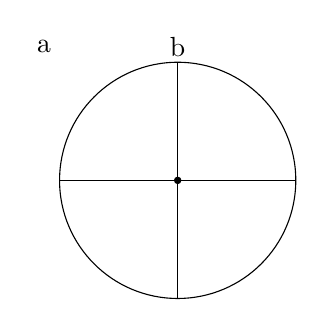
\begin{tikzpicture}
\draw (0,0) circle (1.5cm);
\draw (-1.5,0) -- (1.5,0);
\draw (0,-1.5) -- (0,1.5);
\draw [fill = black] (0, 0) circle (0.04);
\node at (-1.7, 1.7) {a};
\node at (0,1.7) {b};
\end{tikzpicture}
\end{center}

\Rightarrow \left| y \right | \leq r + \left| a \right|

\Rightarrow y^2 \leq (r + \left| a \right|)^2

\text{Same for } y_i, \quad y_i^2 \leq (r + \left|b\right|)^2

\forall z = (x,y) \in D_{a,b}

\left\| z \right\| = \sqrt{x^2 + y^2}

\leq \sqrt{(r + |a|)^2 + (r + |b|)^2}

\text{Thus if } M = \sqrt{(r + |a|)^2 + (r + |b|)^2}, \text{ the bound holds.}

\# \text{IS named boundness = distance boundedness.}

\text{Let } x = (x_1, x_2), y = (y_1, y_2) \in D_{a,b}

z_1 = \{x,y\}^2

(x_2 - a)^2 + (x_2 - b)^2 = r^2

\Rightarrow d(z_1, (a,b)) = \sqrt{(x_2 - a)^2 + (x_2 - b)^2} \leq r

\Rightarrow d(x, y) \leq d(x, (a,b)) + d(y, (a,b))

= \sqrt{(x_1 - a)^2 + (x_2 - b)^2} + \sqrt{(y_1 - a)^2 + (y_2 - b)^2}

\leq r + r = 2r.

\textbf{(iii)} Suppose that $x \neq y$. Then $d(x, y) \neq 0$. Thus if we choose $\epsilon = d(x, y) \Rightarrow \epsilon > 0$ but $d(x, y) \geq \epsilon$. (contradiction).

\textbf{(contradiction)} Suppose $x \neq y$ and so $d(x, y) \neq 0$. 
Choose $\epsilon > 0$ such that $\epsilon = d(x, y)$. Then we must have
$ d(x, y) < \epsilon = \frac{d(x, y)}{2},$
which is a contradiction, as this implies 
if $d(x, y) > 0$ 
$\Rightarrow d(x, y) = \epsilon < \epsilon = \frac{\epsilon}{2} $
$\Rightarrow \epsilon > 0 \Rightarrow \frac{\epsilon}{2}.$
Thus $x = y$. 

\textbf{(iv)} Let $(V, \|\cdot\|)$ be a normed vector space. 

Then let $r > 0$ and $x \in V$. Then
$ B_r(x) = \{u \in V \mid d(x, u) < r\}$
$ B_{\epsilon + \| x \|}(0) = \{ v \in V \mid d(0, v) < \epsilon + \|x\| \}$

\begin{center}
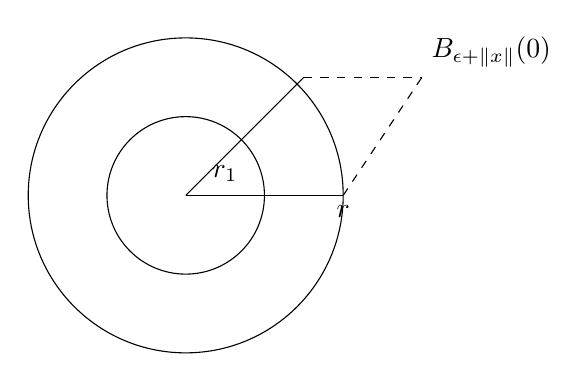
\begin{tikzpicture}
\draw circle (2);
\draw circle (1);
\draw (0,0) -- (2,0);
\draw (0,0) -- (1.5,1.5);
\draw[dashed] (1.5,1.5) -- (3,1.5);
\draw[dashed] (2,0) -- (3,1.5);
\node at (2,0) [below] {$r$};
\node at (0.5,0.5) [below] {$r_1$};
\node at (3,1.5) [above right] {$B_{\epsilon + \| x \|}(0) $};
\end{tikzpicture}
\end{center}

Let $y \in B_r(x)$. 
$ d(0, y) \leq d(0, x) + d(x, y) $
$ \leq \| x \| + r $
$ \Rightarrow B_r(x) \subseteq B_{\epsilon + \| x \|}(0). $

\textbf{(v)} Suppose $S$ is bounded. Then 
$ \exists M \in \mathbb{R} : \forall x \in S \ \|x\| \leq M. $
(Equal to $\exists R \in \mathbb{R} : \forall x \in \mathbb{R}^n$) 
$ x \in B_m(0) $\end{document}